\setchapterpreamble[u]{
    \dictum[La Guía del Autoestopista Intergaláctico]{\raggedleft\textquote{Don't panic}}
}
\chapter{Diseño RTL}

\newcommand{\textmodule}[1]{\texttt{#1}}

Se ha generado un diseño RTL escrito en SystemVerilog con dos partes diferenciadas: una NoC autónoma parametrizable que puede ser conectada en cualquier sistema, y un conjunto de módulos que adaptan la NoC a la unidad de ejecución (EXU) del procesador SweRV-EL2.

Los submódulos de la EXU utilizan la NoC como intermediaria, para enviar las señales de entrada de la EXU al submódulo correspondiente, y las de salida del submódulo a la salida de la EXU.

Para el diseño e implementación del circuito se ha seguido una estrategia de abajo a arriba o \textit{bottom-up}, comenzando con el diseño e implementación de las partes individuales y, una vez simuladas y verificadas, continuando con las partes más grandes que instancian dichos módulos.

\section{Diseño de la Red en Chip}

Se ha especificado una NoC con las características de la sección \ref{sec:especificacion}. La figura \ref{fig:sketch_modules} ilustra un diagrama con los distintos módulos y su jerarquía, siendo los siguientes:
\begin{itemize}[noitemsep]
    \item \textbf{\textmodule{mesh}}: Es la malla encargada de conectar los distintos encaminadores (\textmodule{router}) entre sí, y de proveer un array de puertos de entrada y salida. Es el módulo \textit{top} de la NoC.
    \item \textbf{\textmodule{router}}: Implementa el encaminador, recibe los paquetes de los \textmodule{router}s o dispositivos adyacentes, los procesa, y los reenvía por el puerto correspondiente, haciendo uso de un \textmodule{crossbar}.
    \item \textbf{\textmodule{crossbar}}: Se encarga de la conmutación, permitiendo que el \textmodule{router} realice el encaminamiento.
\end{itemize}

\begin{figure}[h]
    \centering
    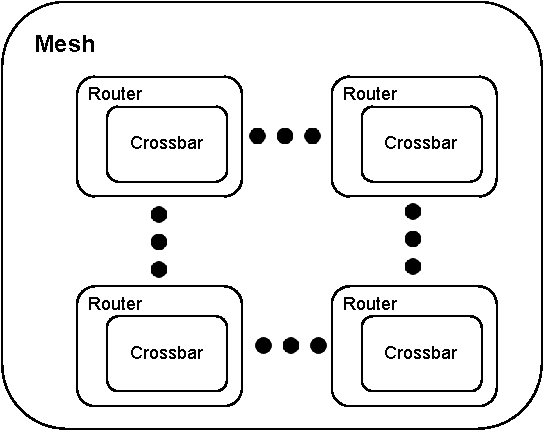
\includegraphics[width=7cm]{images/diagrams/bottom-up.pdf}
    \caption[Diagrama de la jerarquía de módulos de la NoC]{Bosquejo de la jerarquía de módulos de la NoC, siendo \textmodule{mesh} el \textit{top-module}, y pudiendo instanciarse los \textmodule{router} todas las veces que se especifique en los parámetros de la \textmodule{mesh}.}
    \label{fig:sketch_modules}
\end{figure}

En nuestro caso, siguiendo la metodología \textit{bottom-up} hemos diseñado en primer lugar el \textmodule{crossbar}, luego el \textmodule{router}, y después el \textmodule{mesh}. Aun así, durante el diseño de los módulos superiores han surgido nuevos requisitos de los módulos inferiores, por lo que su especificación no ha sido completada hasta finalizar el proyecto.

Durante la implementación se ha intentado parametrizar los diseños para facilitar la reusabilidad de los módulos y reducir la cantidad de código duplicado.

\subsection{Crossbar}

El objetivo de un \textmodule{crossbar} es conectar $n$ entradas con $n$ salidas sin contención. El \textmodule{crossbar}, por lo tanto, recibirá peticiones para conectar un puerto \textit{fuente} con uno \textit{destino} y deberá decidir si cumplirlas o denegarlas. Además, el \textmodule{crossbar} implementado conecta también un camino de \textit{back-propagation} que permite enviar datos desde el puerto \textit{destino} al \textit{fuente}. Si dos puertos piden el mismo destino, se le concederá la conexión únicamente a aquel que tenga mayor prioridad.

Por ejemplo, en un \textmodule{crossbar} de 4 puertos, si las fuentes \textit{0} y \textit{2} intentan establecer una conexión con los destinos \textit{2} y \textit{3}, no se producirá ningún problema y ambas peticiones podrán ser satisfechas. Sin embargo, si a esta situación le añadimos que el puerto \textit{1} pide conectarse a la salida \textit{2}, habrá un conflicto con la petición de \textit{0}, con lo que el \textmodule{crossbar} deberá decidir cual de las dos peticiones cumplir. La figura \ref{fig:crossbar_example} ilustra este ejemplo en el que se ha decidido llevar a cabo la petición de $0$ y denegar la de $1$.

\begin{figure}[h]
    % \centering
    % 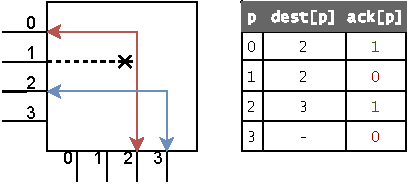
\includegraphics[width=7cm]{images/diagrams/sample_crossbar.drawio.pdf}
    % \caption[Ejemplo de establecimiento de conexiones de un crossbar de cuatro puertos.]{Ejemplo de establecimiento de conexiones de un crossbar de cuatro puertos. Como el puerto \texttt{0} y el puerto \texttt{1} piden la misma salida, solo se establece la conexión con el de mayor prioridad (el \texttt{0})}
    \begin{captionbeside}[Ejemplo de establecimiento de conexiones de un \textmodule{crossbar} de cuatro puertos.]{Ejemplo de establecimiento de conexiones de un \textmodule{crossbar} de cuatro puertos. En la tabla de la derecha, \texttt{p} es el número de puerto, \texttt{dest[p]} el puerto destino pedido por \texttt{p}, y \texttt{ack[p]} la respuesta del \textmodule{crossbar} a esa petición. Como el puerto \texttt{0} y el puerto \texttt{1} piden la misma salida, solo se establece la conexión con el de mayor prioridad (el \texttt{0}).}[l][\linewidth]
        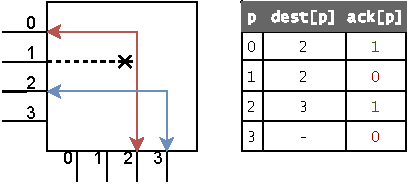
\includegraphics[width=8cm]{images/diagrams/sample_crossbar.drawio.pdf}%
    \end{captionbeside}

    \label{fig:crossbar_example}
\end{figure}

La prioridad, en lugar de estar fija, se establece mediante \textit{round-robin} para evitar el problema de la \textit{espera indefinida} (\autoref{subsec:routing-problems}). El \textmodule{crossbar} tiene un contador módulo $n$ --el número de puertos-- que se aumenta cada ciclo de reloj e indica cual es el puerto de mayor prioridad.

El \textmodule{crossbar} está parametrizado por los siguientes parámetros:
\begin{itemize}[nosep]
    \item \textbf{PORTS}: Número de puertos de entrada y salida del \textmodule{crossbar}.%  Tiene el mismo número de puertos de entrada que de salida. % , por lo que es cuadrado.
    \item \textbf{WIDTH}: Anchura en bits del canal de conexión de la fuente al destino.
    \item \textbf{BP\_WIDTH}: Anchura en bits del canal de conexión inverso (\textit{back-propagation}).
\end{itemize}

Teniendo en cuenta todas las restricciones, y los parámetros, la tabla \ref{tab:crossbar_ports} presenta los puertos del \textmodule{crossbar}.

\begin{table}[h]
    \centering
    \footnotesize
    \begin{tabular}{c|l|l|l|l}
         \hline
         Dir. & \textbf{Tamaño} & \textbf{Puerto} & \textbf{Cantidad} & \textbf{Comentario} \\\hline
         I & 1 & clk & 1 & Reloj de la NoC para el round-robin \\
         I & 1 & rst & 1 & Reset para el registro del round-robin \\
         I & WIDTH & data\_i & PORTS & Los distintos canales de entrada \\
         I & BP\_WIDTH & bp\_data\_i & PORTS & Entrada del back-propagation \\
         I & $\log_2 PORTS$ & dest & PORTS & Petición del puerto de salida \\
         I & 1 & dest\_en & PORTS & Si la petición es válida o no \\
         O & WIDTH & data\_o & PORTS & Datos de salida por cada puerto \\
         O & 1 & data\_o\_en & PORTS & Si los datos de salida son válidos \\
         O & 1 & bp\_o & PORTS & Salida del camino de back-propagation \\
         O & 1 & ack & PORTS & Si se ha asignado la petición de destino \\\hline
    \end{tabular}
    \caption{Puertos del \textit{Crossbar}}
    \label{tab:crossbar_ports}
\end{table}

\subsection{Encaminador}

El módulo \textmodule{router} es el elemento de la red encargado de realizar el encaminamiento de la información. El \textmodule{router} no es más que una pequeña unidad de control que maneja un \textmodule{crossbar} de 4 puertos del ancho del \textit{flit}. Cada \textmodule{router} tiene 4 puertos (Norte, Sur, Este y Oeste) y, por cada puerto, una máquina finita de estados o FSM que representa el estado de la conexión por ese puerto. Como las decisiones de encaminamiento se toman por cada puerto, decimos que el encaminamiento es \textit{distribuido} en lugar de centralizado. La figura \ref{fig:router_fsm} muestra el diagrama de transición de estados de la FSM usada, con los siguientes estados:
\begin{itemize}
    \item \textbf{\textit{IDLE}}: Aún no se está enviando información por este puerto. En el caso en el que nos llegue una cabecera, de manera combinacional aplica \textit{Dimensional Order Routing} para calcular el puerto de destino y comprueba en los registros de destino de los otros puertos si ningún otro \textmodule{router} lo está usando. En caso de que entren dos cabeceras a la vez con el mismo destino, el \textmodule{crossbar} deberá encargarse de realizar el arbitraje. El puerto para el que el \textmodule{crossbar} haya cumplido la petición pasará al estado \textit{ESTABLISHING}, guardando la información de destino en un registro y bloqueando la salida por ese puerto.
    \item \textbf{\textit{ESTABLISHING}}: Como el establecimiento del circuito virtual está segmentado, la cabecera debe seguir propagándose por los nodos intermedios hasta el ciclo en el que se reciba un \textit{ack} por su puerto de \textit{back-propagation}, momento en el cual podemos pasar a enviar la información.
    \item \textbf{\textit{ESTABLISHED}}: La conexión ha sido establecida y solo es necesario mantener la conmutación, hasta que se reciba un flit de tipo \textit{TAIL}, que liberará los recursos haciendo que el puerto pase al estado \textit{IDLE} de nuevo.
\end{itemize}

\begin{figure}[h]
    \centering
    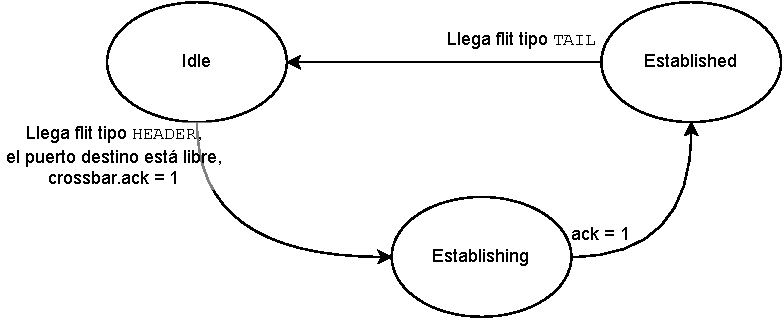
\includegraphics[width=12cm]{images/diagrams/router_fsm.drawio.pdf}
    \caption[Máquina de Estados Finita del puerto de un encaminador.]{FSM del puerto de un \textmodule{router}.}
    \label{fig:router_fsm}
\end{figure}

Para que sea posible realizar el encaminamiento, debido a que el direccionamiento es \textit{absoluto}, el \textmodule{router} debe recibir por parámetro su posición $(x,y)$ dentro de la red. Además, para evitar mandar paquetes por el \textit{borde} (donde no hay \textmodule{routers}), recibe la posición máxima hasta la que puede encaminar.

Las entradas y salidas del encaminador son simplemente el reloj de la NoC, una señal de reset global asíncrona para los registros de la FSM, y 4 puertos de entrada y 4 de salida del tipo interfaz \textit{node\_port}, explicado en la siguiente subsección.

\subsection{Interfaz puerto}

En SystemVerilog, una interfaz es una manera de encapsular un conjunto de señales relacionadas en un bloque, para que pueda ser instanciada y reusada a lo largo del proyecto, facilitando el desarrollo y minimizando los problemas al realizar cambios \cite{CVSVIface}.
% Las entradas y salidas del encaminador son simplemente el reloj de la NoC, una señal de reset global asíncrona para los registros de la FSM, y 4 puertos de entrada y 4 de salida de tipo interfaz \textit{node\_port}. 

Para codificar el tipo de las entradas/salidas de los puertos de los elementos de la red se ha decidido usar una \textit{interfaz} de SystemVerilog. De esta manera, al crear un módulo que use dichas señales, tan solo es necesario poner como puerto esta interfaz. Por ejemplo, si se añadiese una nueva señal de control a la comunicación, no sería necesario cambiar la descripción del módulo \textmodule{mesh}.

Las interfaces de SystemVerilog permiten definir \textit{modports}, en los que se especifica la dirección de las señales. Una misma interfaz puede tener varios \textit{modports} para especificar las distintas ``perspectivas'' que pueden tener distintos componentes al usar esa interfaz.

En nuestro caso, se define un \textit{modport} \textit{down} (de \textit{downlink} o \textit{download}) que usarán los dispositivos que puedan recibir información de la red. Los dispositivos que deseen enviar información deben declarar el puerto usando el \textit{modport} \textit{up} (de \textit{uplink} o \textit{upload}), en el que se cambia la dirección de todas las señales.

Finalmente, en la tabla \ref{tab:port_iface_ports} se muestran las señales que definen la interfaz \textmodule{node\_port}, desde el \textit{punto de vista} de un dispositivo que recibe un flit (modport \textit{down}).

\begin{table}[h]
    \centering
    \footnotesize
    \begin{tabular}{c|l|l|l}
         \hline
         \textbf{Dir.} & \textbf{Tipo} & \textbf{Nombre} & \textbf{Descripción} \\\hline
         I & flit\_t & flit & El flit a enviar \\
         I & logic   & enable & Si queremos habilitar la conexión (la información en \textit{flit} es válida) \\
         O & logic   & ack & Si se ha conseguido establecer una conexión \\\hline
    \end{tabular}
    \caption{Puertos de la interfaz \textmodule{node\_port} con modport \textit{down} (entrada de datos).}
    \label{tab:port_iface_ports}
\end{table}

\subsection{Malla}
El módulo \textmodule{mesh} instancia los distintos \textmodule{router} y los conecta entre ellos formando una malla bidimensional. Sus entradas son un reloj y un reset global asíncrono que será pasado a cada uno de los nodos. Además, expone arrays de interfaces de tipo \textmodule{node\_port} a lo largo de su perímetro, por lo que tiene un total de $2\cdot \left(WIDTH+HEIGHT\right)$ \textmodule{node\_port}s de entrada (\textit{down}), y otros tantos de salida (\textit{up}).

Para ello, recibe por parámetro el ancho y alto deseado y, usando bucles \textit{generate} de SystemVerilog, instancia los nodos y sus conexiones. Al igual que se creó la interfaz \textmodule{node\_port} para facilitar la implementación de la malla, se ha creado un módulo \textmodule{node\_link}, que se encarga simplemente de recibir dos interfaces de tipo \textmodule{node\_port} y conectarlas combinacionalmente. 

Instanciando estos módulos enlace cada vez que queramos conectar dos puertos, hacemos que si cambiamos el interfaz \textmodule{node\_port} solo haga falta cambiar el código de las conexiones una única vez en el módulo \textmodule{node\_link}, sin ser necesario modificar el código de la malla.

\subsection{Simulación y validación}
\label{subsec:rtl_simulacion}
Para comprobar la resiliencia de la red ante diversos estímulos, en lugar de usar señales generadas a mano con inspección manual de las salidas, se ha creado un testbench con auto-comprobaciones.

Las pruebas consisten en la generación de una serie de \textit{Paquetes} de manera aleatoria (fuente, destino y datos) a lo largo del tiempo que serán encolados y enviados por las distintas entradas de la red, comprobando que, eventualmente, llegan a su destino. La idea es simular una serie de computadores que generan paquetes de tamaño aleatorio (siguiendo una distribución uniforme), con una probabilidad $p$ de que cada dispositivo genere un paquete en un momento dado.

Para simular distintas condiciones de red, la probabilidad $p$ va cambiando a lo largo de la simulación, aunque es la misma para todos los dispositivos. Durante los primeros $30000$ ciclos de reloj, la probabilidad de que un dispositivo genere un paquete es fija y es de $0.01\%$.
% Como en cada ciclo se calcula esta probabilidad para todos los dispositivos, si queremos calcular la probabilidad en total de que se genere un paquete (en cualquier dispositivo) ha. 
Nótese que cada ciclo de reloj se calcula esa probabilidad para cada uno de los emisores, por lo que la probabilidad de que en un ciclo se genere un paquete es mayor, y para calcularla hay que tener en cuenta las dimensiones de la red.
A partir de los $30000$ ciclos, $p$ se aumenta linealmente a un ritmo de $0.01\%$ cada $100$, hasta llegar a la saturación de la red (cuando la cola del generador está llena). Momento en el que se dejan de enviar paquetes y, eventualmente, debería vaciarse la red.

El campo de pruebas cuenta con los siguientes procesos concurrentes (visualizados en la figura \ref{fig:diagram_testbench}):
\begin{itemize}[nosep]
    \item Un \textbf{generador} de paquetes que, por cada ciclo de reloj, genera distintos paquetes con su fuente y destino con probabilidad $p$, y los envía a la cola de los emisores y los receptores correspondientes.
    \item Tantos \textbf{emisores} como puertos de entrada tiene la NoC. Van consumiendo paquetes de la cola, troceándolos en flits, y enviandolos por la red respetando el protocolo de transmisión. También es capaz de detectar bloqueos contando el número de ciclos necesarios para establecer una conexión. Si ese número de ciclos es mayor que una constante, lanza un \textit{warning}.
    \item Tantos \textbf{receptores} como puertos de salida tiene la malla. Comprueban que los paquetes que le llegan son para ese destino, y que han sido emitidos previamente. Para ello, tienen una lista con los flits generados por el generador con este destino. Al terminar el test, si todavía quedan paquetes en dicha lista, es porque han sido emitidos pero no recibidos (perdidos), por lo que se imprimen y el test acaba con errores.
\end{itemize}

\begin{figure}[h]
    \centering
    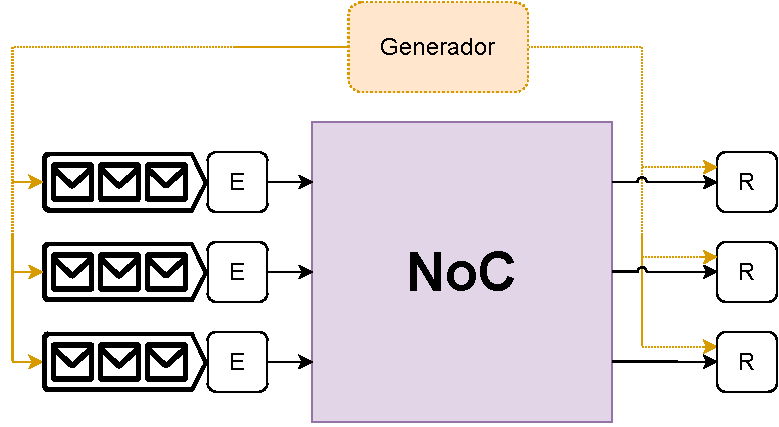
\includegraphics{images/diagrams/testbench.drawio.pdf}
    \caption[Diagrama del funcionamiento del \textit{testbench}.]{Representación del funcionamiento del \textit{testbench}. Existen tantos emisores (E) como receptores (R), uno por cada puerto de entrada o salida de la red.}
    \label{fig:diagram_testbench}
\end{figure}

La ejecución de la simulación genera una serie de ficheros en formato de tabla separado por comas (CSV) que pueden ser procesados con herramientas externas para obtener más información del estado de la red durante la simulación. La tabla \ref{tab:csv_tables} muestra los datos de los paquetes incluidos en los CSV. Los resultados de la simulación y el análisis de los datos generados se presentan en la sección \ref{sec:resNoC}

\begin{table}[ht]
    \centering
    \begin{subtable}[t]{\textwidth}
        \centering
        \begin{tabularx}{.8\textwidth}{ c | X }
            \hline
            \textbf{Nombre} & \textbf{Descripción} \\
            \hline
            p\_id & identificador del paquete \\
            gen\_cycle & ciclo en el que se genera el paquete \\
            src\_x & ordenada x de la fuente del paquete \\
            src\_y & ordenada y de la fuente del paquete \\
            dst\_x & ordenada x del destino del paquete \\
            dst\_y & ordenada y del destino del paquete \\
            p\_size & Tamaño de los datos del paquete \\
            prob & La probabilidad de generar un paquete \\
            \hline
        \end{tabularx}
        \caption{Columnas del CSV creado por el proceso \textit{generador}.}
    \end{subtable}
    \begin{subtable}[t]{\textwidth}
        \centering
        \begin{tabularx}{.8\textwidth}{c|X}
            \hline
            \textbf{Nombre} & \textbf{Descripción} \\
            \hline
            p\_id & identificador del paquete \\
            hdr\_cycle & ciclo en el que comienza la emisión de la cabecera \\
            sending\_cycle & ciclo en el que comienza la emisión de datos \\
            tail\_sent\_cycle & ciclo en el que finaliza la emisión de datos \\
            \hline
        \end{tabularx}
        \caption{Columnas del CSV escrito por los procesos \textit{emisores}.}
    \end{subtable}
    \caption{Columnas de los ficheros CSV \textit{packets.csv} y \textit{senders.csv}, modificados por el \textit{generador} y los \textit{emisores} respectivamente.}
    \label{tab:csv_tables}
\end{table}

\subsection{Envoltorio post-síntesis}
La síntesis con Vivado tiene ciertas restricciones. Para hacer que los módulos sean compatibles con herramientas que reciben \textit{stubs} de Verilog, como este no soporta arrays ni interfaces, el sintetizador modifica el nombre de las señales de entrada/salida de nuestros módulos para hacerlos compatibles. En consecuencia, se ``aplanan'' los arrays, generando una señal por cada uno de los elementos de nuestro array. Como efecto secundario, esto hace que nuestro \textit{testbench}, que era válido para pruebas de comportamiento, ya no sea compatible con el modelo sintetizado debido al cambio en el nombre de las señales.

Para solucionar este problema se ha creado un envoltorio (\textit{wrapper}) que, dependiendo de una constante de compilación, utiliza el nombre de las señales originales (para simulación pre-síntesis), o ``convierte'' el nombre de las señales usando \textit{assigns} y \textit{wires}. Debido a que es necesario generar tantas señales nuevas como elementos hubiese en los arrays de los puertos de la NoC, se ha creado un pequeño \textit{script} en Python que genera parte de este envoltorio. Sin embargo, como el wrapper recibe el tamaño de la NoC por parámetro para pasárselo a la malla, el código generado por el script contiene condicionales de tiempo de compilación para evitar tener que regenerar el wrapper usando el script cada vez que cambiemos el tamaño de la red.

\section{Integración de la NoC en el SweRV-EL2}
La NoC se usa dentro del RISC-V para conectar distintos elementos de la unidad de ejecución (EXU). En su configuración original, estas conexiones son buses de señales punto a punto. Por lo tanto, ha sido necesario generar módulos que conviertan estas señales a paquetes, y los transmitan/reciban por la red siguiendo el protocolo especificado en la sección \ref{subsec:noc_protocolo}.

\subsection{Emisor}
\label{subsec:emisor}
El módulo \textmodule{sender} se encarga de recibir un bus de longitud preestablecida, empaquetarlo en flits y enviarlo por la red a un receptor. Para disminuir la cantidad de flits a enviar, es posible enviar una cantidad reducida de bits en el espacio libre de la cabecera.

El módulo tiene dos parámetros: \textbf{PACKET\_BITS} que establece la longitud de los bits a ser enviados en el paquete y \textbf{PADDING\_BITS} que establece la longitud de los bits a ser enviados en la cabecera, y debe ser menor que la cantidad de bits en la parte libre de la cabecera. Automáticamente se calcula un parámetro local con el número de flits a enviar, dividiendo \textit{PACKET\_BITS} por la cantidad de bits por flit.

Para enviar un paquete, se habilita la señal \textit{enable}, comenzando la emisión de los datos de los buses de entrada. Una vez se han enviado todos los flits que forman un paquete, se pone a 1 la señal de salida \textit{ack}. Si queremos enviar otro paquete primero es necesario establecer a 1 la entrada \textit{flush} para indicar que los datos de entrada han cambiado y puede volverse a emitir el mensaje. Los puertos de entrada y salida del módulo quedan definidos en la tabla \ref{tab:sender_ports}.

Para mantener el diseño lo más sencillo posible y minimizar la cantidad de registros necesarios, es imprescindible que las entradas permanezcan estables durante la emisión del paquete, pues no se guardan en registros.

\begin{table}[h]
    \centering
    \footnotesize
    \begin{tabular}{c|l|l|l}
         \hline
         \textbf{Dir.} & \textbf{Tipo} & \textbf{Nombre} & \textbf{Descripción} \\\hline
         I & logic & clk & El reloj de la red \\
         I & logic & rst & Reset asíncrono para los registros de la FSM \\
         I & logic & enable & Podemos comenzar la emisión \\
         I & logic & flush  & Queremos enviar nuevos datos de entrada \\
         I & logic & dst\_addr & La dirección a la que enviar los datos \\
         I & [PADDING\_BITS] & padding & Los bits a embeber en la cabecera \\
         I & [PACKET\_BITS] & packet & Los bits a empaquetar y enviar tras la cabecera \\
         O & logic   & ack & Si se ha conseguido enviar el paquete \\
         O & node\_port & up & El puerto de salida a conectar con la NoC \\\hline
    \end{tabular}
    \caption{Puertos de un \textit{serial sender}.}
    \label{tab:sender_ports}
\end{table}
\begin{figure}[h]
    \centering
    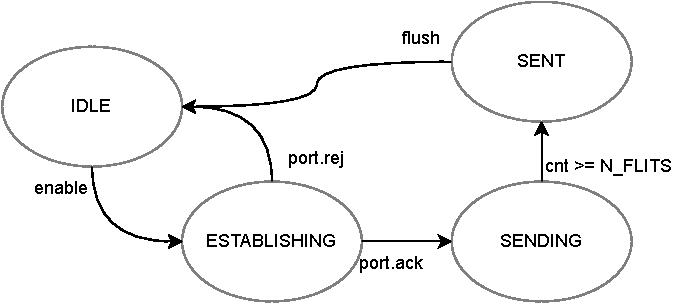
\includegraphics[width=10cm]{images/diagrams/sender_fsm.drawio.pdf}
    \caption[Máquina de Estados del emisor de datos recibidos en serie.]{FSM del emisor de datos recibidos en serie.}
    \label{fig:sender_fsm}
\end{figure}

La figura \ref{fig:sender_fsm} presenta el diagrama de transición de estados de la FSM del emisor, que cuenta con los siguientes estados:

\begin{itemize}
    \item \textbf{\textit{IDLE}}: No se están enviando datos. Si se activa \textit{enable}, pasa a \textit{ESTABLISHING} y comienza el envío de la cabecera.
    \item \textbf{\textit{ESTABLISHING}}: Se establece el camino. Para ello, se reenvía la cabecera hasta recibir el \textit{ack} de la conexión, con lo que pasa al estado \textit{SENDING}.
    \item \textbf{\textit{SENDING}}: Se envían el resto de flits que forman el paquete. La cantidad de flits \textit{N\_FLITS} es constante, y es simplemente el número de bits a enviar dividido por los bits que caben en cada flit. Nos mantenemos en este estado hasta que hayamos enviado todos los flits, tras lo cual pasa al estado \textit{SENT}.
    \item \textbf{\textit{SENT}}: La emisión queda bloqueada hasta que se reciba la señal \textit{flush}, enviada por el usuario del emisor, haciendo que el emisor sea \textit{one-shot}.
\end{itemize}

\subsection{Receptor}
\label{subsec:receptor}
El receptor tiene un diseño similar al emisor, si bien su tarea es precisamente la contraria. Se encarga de recibir un paquete, dividido en flits, que ha sido enviado por un emisor y desplegarlo en un bus. Tiene, por lo tanto, los mismos parámetros que el emisor (véase \ref{subsec:emisor}) y un funcionamiento similar. La tabla \ref{tab:receiver_ports} muestra los puertos de entrada y salida de este módulo.

Cuando el receptor ha terminado de recibir un paquete y este está disponible en los puertos \textit{padding} y \textit{packet}, pone la señal de salida \textit{valid} a 1. Una vez se haya consumido este dato, el módulo usuario debe poner la señal de \textit{flush} a 1 para que se pueda recibir otro paquete.

\begin{table}[h]
    \centering
    \footnotesize
    \begin{tabular}{c|l|l|l}
        \hline
        \textbf{Dir.} & \textbf{Tipo} & \textbf{Nombre} & \textbf{Descripción} \\\hline
        I & logic & clk   & Reloj de la red \\
        I & logic & rst   & Reset asíncrono para los registros de la FSM \\
        I & logic & flush & Liberar los recursos \\
        I & node\_port & down & Puerto de entrada a conectar con la NoC \\
        O & logic & valid & Si \textit{padding} y \textit{packet} son válidos \\
        O & [PADDING\_BITS] & padding & Los bits embebidos en la cabecera \\
        O & [PACKET\_BITS] & packet & Los bits recibidos en el cuerpo de los flits \\\hline
    \end{tabular}
    \caption{Puertos de un \textit{serial receiver}.}
    \label{tab:receiver_ports}
\end{table}

La figura \ref{fig:receiver_fsm} presenta la FSM del \textmodule{receiver}, que cuenta con un estado menos que el \textmodule{sender}:
\begin{itemize}
    \item \textbf{\textit{IDLE}}: Los recursos están disponibles y se puede recibir información. Con la salida \textit{down.ack} a $1$ se señaliza al \textit{router} conectado que es posible recibir datos. Al recibir una cabecera, se almacenan en un registro los \textit{PADDING\_BITS}, pasando al estado \textit{RECEIVING}.
    \item \textbf{\textit{RECEIVING}}: Debido a la conmutación de circuitos segmentada es posible recibir la cabecera repetida, por lo que es necesario ignorarla hasta recibir el primer flit de datos. Después, se almacena la carga de los \textit{flits} de datos recibidos en el registro correspondiente hasta recibir un flit de tipo TAIL, pasando al estado \textit{VALID}. Para saber qué registro habilitar, se usa un contador del número de flits de datos recibidos, que será la entrada de un decodificador cuya salida serán las señales \textit{enable} de cada uno de los registros que almacenan la salida \textit{packet}. Es decir, aunque todos los registros reciben la misma entrada (los datos del flit), solo se escribe en el registro necesario.
    \item \textbf{\textit{VALID}}: La información del paquete está disponible en las salidas \textit{padding} y \textit{packet}. Se espera a que la salida sea consumida hasta que el usuario del módulo habilite la señal de \textit{flush} para poder recibir paquetes de nuevo. Durante este estado la salida \textit{down.ack} permanece desactivada para que el nodo adyacente no establezca conexiones con este dispositivo, evitando que se pierdan los paquetes o se sobreescriban los registros.
\end{itemize}

\begin{figure}[h]
    \centering
    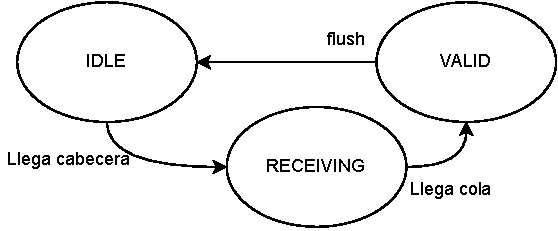
\includegraphics{images/diagrams/receiver_fsm.drawio.pdf}
    \caption[Diagrama de la Máquina de Estados del receptor y desempaquetador de datos]{Diagrama de la FSM del receptor y desempaquetador de datos.}
    \label{fig:receiver_fsm}
\end{figure}
\begin{figure}[ht]
    \centering
    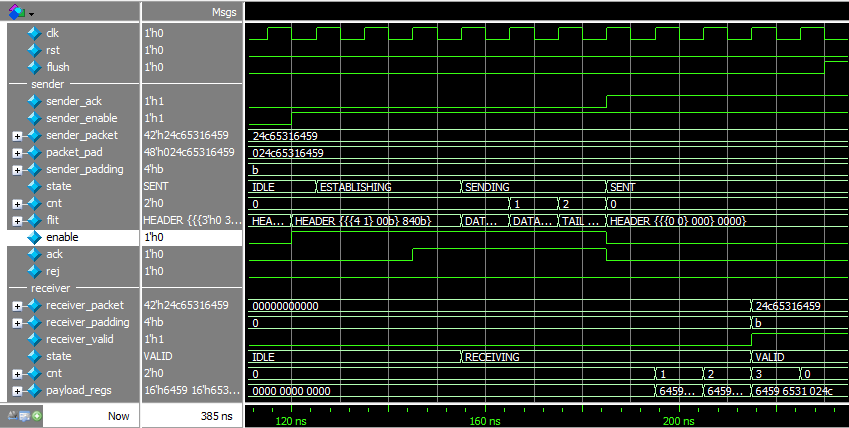
\includegraphics[width=\linewidth]{images/signals/signals_receiver_sender.png}
    \caption[Señales de entrada y salida receptor y emisor en serie]{Señales de entrada y salida de un banco de pruebas con un emisor y un receptor, enviando un paquete de 3 flits a una distancia de 3 nodos. Nótese como los datos enviados en la señal \textit{sender\_packet} acaban siendo replicados en la salida \textit{receiver\_packet}.}
    \label{fig:signals_receiver_senders}
\end{figure}

En conjunto, el emisor y el receptor permiten enviar datos flit a flit a través de la NoC. En la figura \ref{fig:signals_receiver_senders} se muestra el diagrama de señales de una emisión de 42 bits de datos (3 flits y cabecera) a través de una red pasando por tres nodos. Debido a la conmutación de circuitos segmentada, como el paquete pasa por tres nodos, es necesario que el emisor replique la cabecera tres veces hasta recibir el \textit{ack}, permaneciendo en el estado \textit{ESTABLISHING}. El receptor pasa al estado \textit{RECEIVING} el mismo ciclo de reloj que el emisor pasa al estado \textit{SENDING}, sin embargo, el receptor debe descartar la cabecera durante los 3 primeros ciclos. A continuación permanece en dicho estado mientras recibe los 42 bits del paquete (3 flits). 

Puede observarse el momento en el que el receptor deja de descartar cabeceras y empieza a consumir flits de datos observando cuando aumenta la señal \textit{cnt} del \textit{receiver}. Finalmente, tras recibir los tres flits de datos del paquete se pasa al estado \textit{VALID}, desplegando los bits en la señal \textit{receiver\_packet} (que es igual a \textit{sender\_packet}), y habilitando \textit{receiver\_valid}.

\subsection{Wrappers en la unidad de ejecución}

Se han creado distintos \textit{wrappers} que encapsulan cada uno un elemento de la unidad de ejecución. De esta forma, se crea un módulo que se conecta únicamente con la red y que mantiene el mismo comportamiento que el elemento al que envuelve.

Usando el receptor y el emisor mencionados en las secciones anteriores podemos convertir los paquetes de la red a señales del módulo a envolver, y los resultados de ese módulo de nuevo a paquetes.

En la figura \ref{fig:schematic_div_wrapper}, el receptor \textmodule{i\_receiver} desempaqueta los flits recibidos por el puerto \textit{down.flit}, y los pasa a las entradas \textit{dividendo} y \textit{divisor} del módulo \textmodule{divisor}. Cuando el divisor termina de realizar los cálculos, se envía el resultado (\textit{out}) al emisor \textmodule{i\_sender}, que lo empaqueta y lo manda de nuevo por la red.

Para que el envoltorio del divisor pueda recibir y enviar datos a las otras unidades del procesador, es necesario un emisor y receptor encargados de transformar estas señales y mandárselas al wrapper, como podemos ver en la figura \ref{fig:sketch_wrappers}.

\begin{figure}[h]
    \centering
    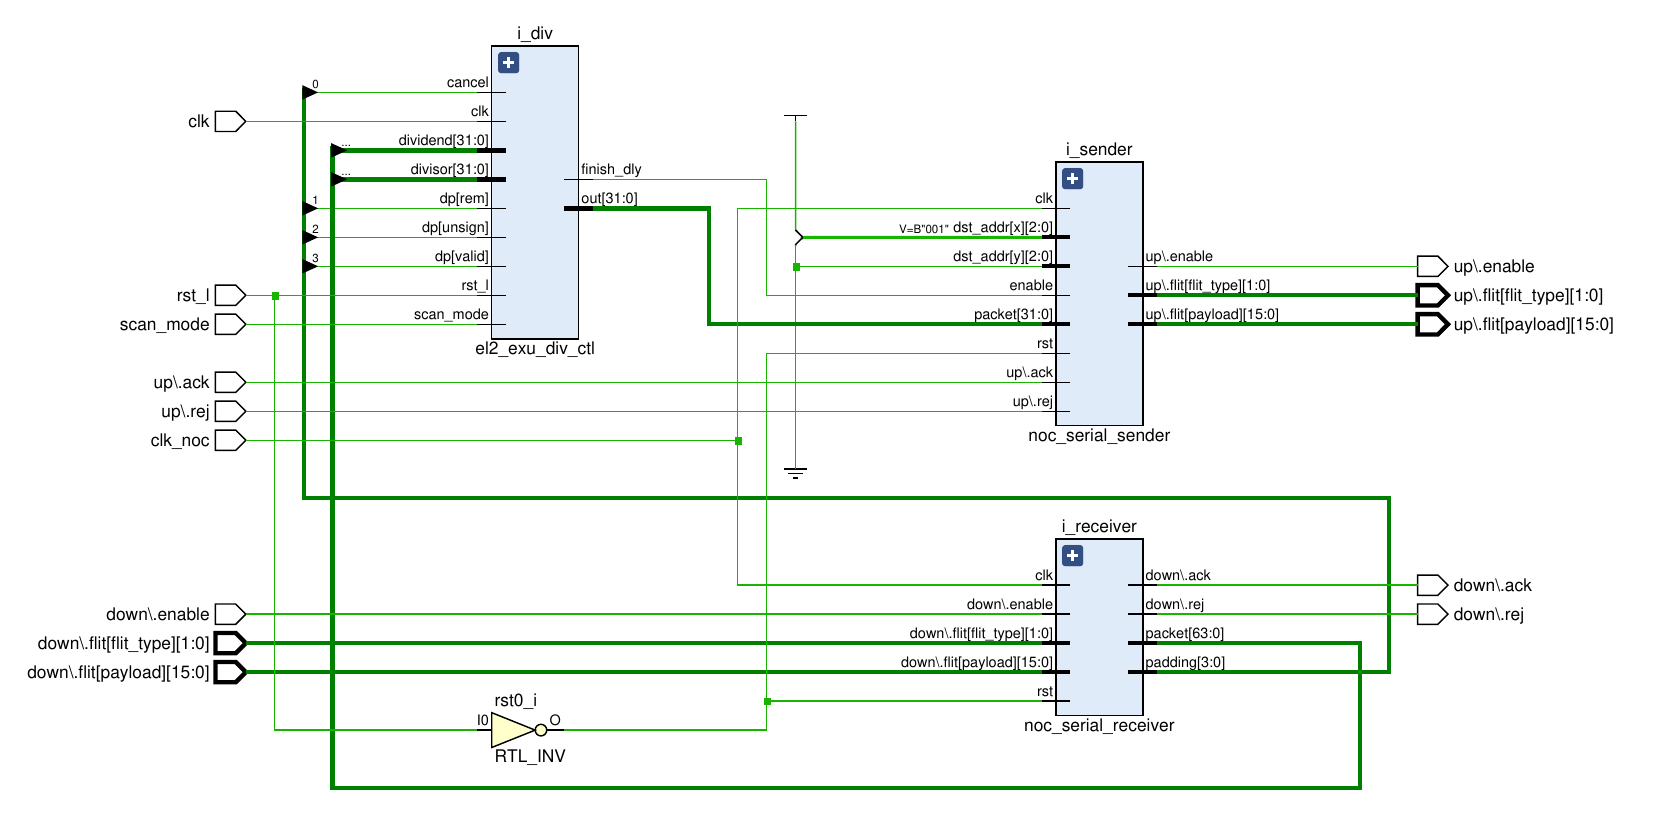
\includegraphics[width=\linewidth]{images/schematics/div_wrapper.png}
    \caption[Diagrama de bloques del módulo \textit{div\_wrapper}]{Diagrama de bloques del módulo \textit{div\_wrapper}, envoltorio del divisor.}
    \label{fig:schematic_div_wrapper}
\end{figure}

\subsection{Modificaciones en la unidad de ejecución}
\label{subsec:exu_mods}
La unidad de ejecución del SweRV-EL2 (EXU o \textit{Execution Unit}) se encarga principalmente de la fase de ejecución de las instrucciones, por lo que recibe los datos con los que operar (extraídos por las fases de \textit{fetch} y \textit{decode}) y devuelve el resultado de la operación (que será usado en la fase de \textit{retire}). Asimismo, la EXU se encarga también de otras operaciones no explicitadas en una instrucción, como predicciones de salto o cálculos relativos al contador del programa. 

Para ello, la unidad de ejecución instancia los siguientes módulos:

\begin{itemize}
    \item \textbf{i\_alu}: Es la Unidad Aritmético Lógica (ALU) y se encarga de hacer operaciones sencillas en menos de un ciclo de reloj, como pueden ser sumas y restas. Es usada para la ejecución de instrucciones aritmético-lógicas, pero también para operaciones con el contador de programa y de predicción de salto.
    \item \textbf{i\_mul}: Se encarga únicamente de realizar multiplicaciones, implementando la extensión \textit{M} del ISA. El resultado está disponible en el siguiente ciclo.
    \item \textbf{i\_div}: A diferencia de los dos anteriores, este dispositivo se encuentra fuera del pipeline principal (decimos que es \textit{out-of-pipe}) y tiene 34 ciclos de latencia. No está segmentado ni tiene cortocircuitos dentro de la ALU.
\end{itemize}

% \begin{figure}[h]
%     \begin{captionbeside}{Flujo de una instrucción y situación de la NoC en dicho flujo.}[l][\linewidth]
%         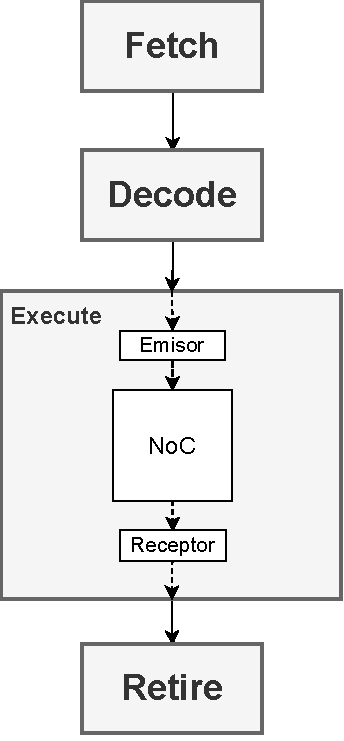
\includegraphics[width=.3\textwidth]{images/diagrams/risc_noc.drawio.pdf}
%     \end{captionbeside}
% \end{figure}
\begin{figure}[h]
    \begin{captionbeside}[Diagrama de bloques de la unidad de ejecución.]{Diagrama de bloques de la unidad de ejecución y los módulos necesarios para el funcionamiento del multiplicador y divisor.}[r][\linewidth]
        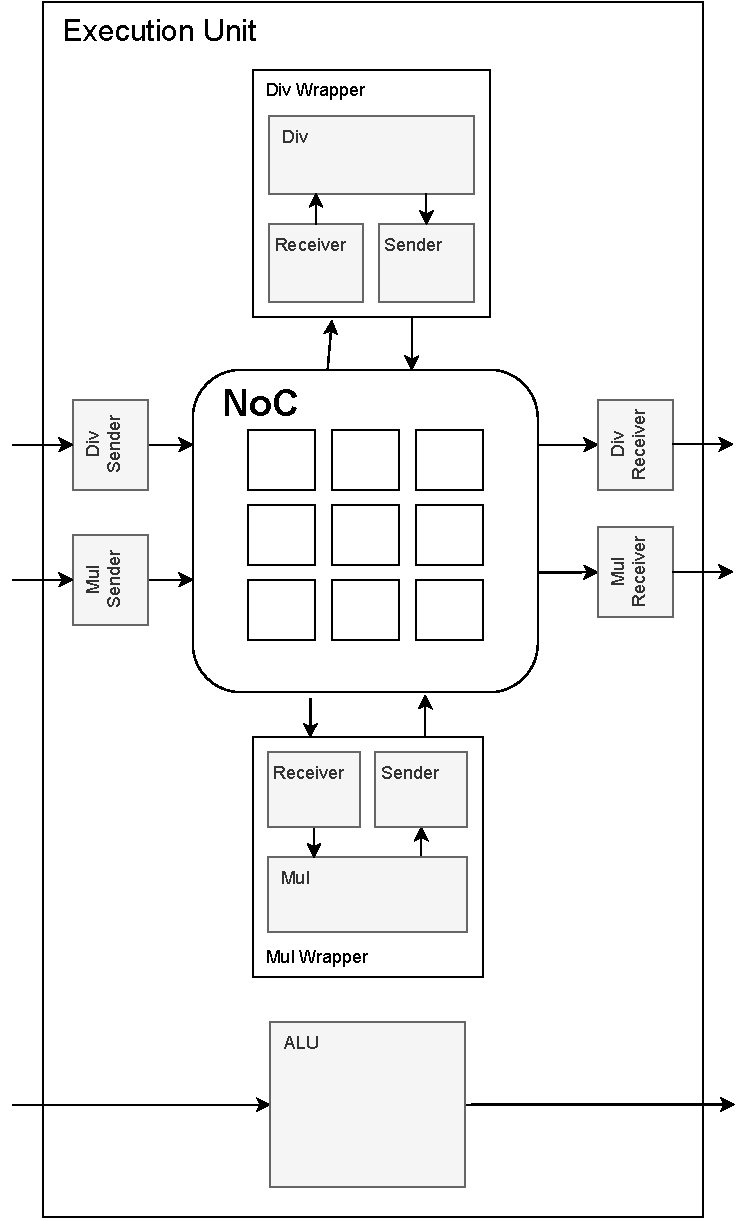
\includegraphics[width=.6\linewidth]{images/diagrams/sketch_wrappers.drawio.pdf}%
    \end{captionbeside}
    \label{fig:sketch_wrappers}
\end{figure}

En este proyecto se ha añadido una NoC a la unidad de ejecución. Debido a que la NoC (definida en el capítulo \ref{chap:desNoC}) necesita de varios ciclos de reloj para enviar un paquete, ha sido necesario añadir un nuevo reloj interno \textit{clk\_noc} que recibe cada uno de los elementos que conforman la NoC, incluidos los emisores y receptores. En las pruebas realizadas, dicho reloj va 16 veces más rápido que el reloj del sistema.

Además, se ha instanciado una malla de tamaño $3\times 3$ (configurable con definiciones del precompilador), y se han instanciado los emisores, receptores y \textit{wrappers} correspondientes alrededor de la NoC para el multiplicador y el divisor, creando paquetes con las siguientes características:

\begin{itemize}
    \item \textbf{Entrada MUL}: Recibe los dos operandos de 32 bits, y un estructurado de 23 bits con información sobre la operación a realizar (si es válida, el signo, etc...). Por lo tanto, el paquete generado tiene $\lceil\frac{32+32+23}{FLIT\_DATA\_WIDTH}\rceil = 6$ flits de datos a 16 bits cada uno.
    \item \textbf{Salida MUL}: Se envía un resultado de 32 bits, por lo que tendremos 2 flits de datos. Dentro del \textit{wrapper}, para evitar enviar siempre el resultado (aunque no se haya hecho ningún cómputo), como el multiplicador no expone ninguna señal de valid, activamos el \textit{enable} del emisor un ciclo después de que entrasen datos al multiplicador, evitando así la sobrecarga de la red.
    \item \textbf{Entrada DIV}: Se envía el numerador y el denominador (de 32 bits), y un estructurado de 3 bits con información de la operación (el signo, y si queremos el cociente o el resto). Como dicho estructurado tiene solo 3 bits, podemos enviarlo en los bits libres de la cabecera, y hacemos que se necesiten tan solo 4 flits de datos para enviar entre el emisor y el \textit{wrapper}.
    \item \textbf{Salida DIV}: Se envía el resultado y una señal que indica que la división ha acabado (pues el divisor es \textit{out-of-pipe}). En lugar de mandar esta señal en el paquete, la usamos para activar el emisor del \textit{wrapper}, y es el receptor el que se encarga de activarla al recibirlo (usando la señal \textit{valid} del módulo \textit{serial\_sender}). Por lo tanto, este resultado necesita de 2 flits de datos para enviarse.
\end{itemize}

Es decir, \textbf{el tamaño máximo de un paquete que pasará por nuestra red es de 7 flits} contando la cabecera, siendo datos para una multiplicación.

En cuanto a la ALU, se ha decidido no incluirla en la NoC debido a su complejo funcionamiento por sus múltiples responsabilidades. Sería necesario realizar numerosas modificaciones para adaptarla, expuestas en el capítulo \ref{chap:trabajo_futuro}.

Todos estos cambios han sido parametrizados con una definición del precompilador \texttt{`RV\_EXU\_NOC}, que nos permite decidir en tiempo de compilación si queremos o no que la EXU utilice la NoC sin ser necesario tener dos proyectos distintos.

\subsubsection{Detector de cambios en reloj}

Como hemos explicado en sus respectivas secciones, el emisor y el receptor son \textit{one-shot}, es decir, tras realizar su acción se bloquean hasta recibir una señal de desbloqueo llamada \textit{flush}.

En el caso del RISC-V con el objetivo de mandar las nuevas señales que pueden haberse generado este ciclo de reloj es necesario mandar la señal de \textit{flush} cuando estas cambien. Para ello se ha creado un detector de cambio de reloj. Este módulo recibe el reloj del que queremos detectar el \textit{rising edge} y un reloj base en el que apoyarnos y que alimentará la lógica secuencial del detector. El módulo tendrá como salida una señal \textit{rising} que se pondrá a uno cuando se detecte un cambio de $0\rightarrow1$ en el reloj principal.

La idea principal es guardar en un registro el estado de la señal el ciclo anterior, y compararla con el estado actual para comprobar si se ha producido un cambio. Esta comparación es simplemente la conjunción lógica, por lo que la salida de nuestro módulo será dada por la fórmula $rising = clk\_slow\ \& ~q$, donde $q$ es el registro con la señal desfasada.

\begin{figure}[h]
    \centering
    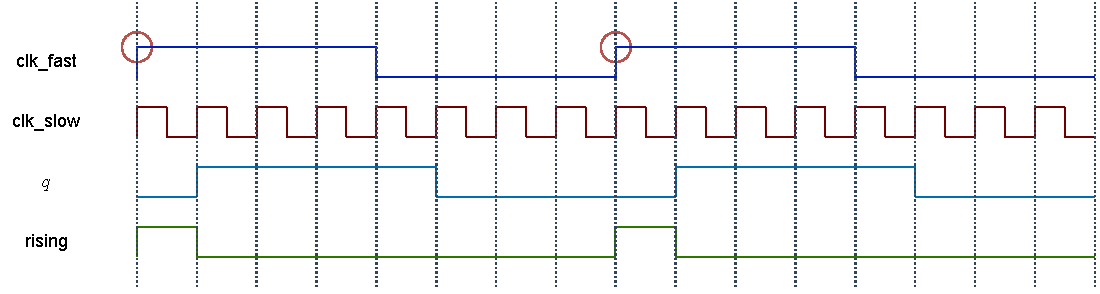
\includegraphics[width=\textwidth]{images/diagrams/edge_detector.drawio.pdf}
    \caption[Diagrama temporal de las señales de un detector de cambios de reloj.]{Diagrama temporal de las señales de un detector de cambios de reloj, con un reloj del que detectar el cambio (\textit{clk\_fast}) 4 veces más lento que el base (\textit{clk\_slow}). También se visualiza la señal interna $q$.}
    \label{fig:signals_edge_detector}
\end{figure}